\documentclass[10pt]{article}
\usepackage[margin=1in]{geometry}
\usepackage{amsmath,amssymb,booktabs,enumitem,graphicx,hyperref,tabularx}
\title{Task-Aware Progressive Retrieval Attention:\\Virtualizing Interleaved Agent Context by Execution Scope}
\author{PRA Research Program}
\date{August 2026}

\begin{document}
\maketitle

\begin{abstract}
Progressive Retrieval Attention (PRA) has largely been studied under an implicit single-task assumption: one physical session is treated as one coherent retrieval space. Long-running agents instead multiplex tasks whose user turns, tool results, artifacts, and decisions are temporally interleaved. We introduce task-aware PRA, where harness-authoritative task identity and dependency relations scope candidates before ordinary PRA discovery and Paper-7 progressive materialization. The implementation provides versioned task events, idempotent DAG replay, typed task provenance, cold/warm/hot working-set transitions, and in-memory and local persistent session services. A controlled oracle experiment spans 80 workflows, four workflow families, 2--16 tasks, and five seeds. At a matched two-record budget in the 16-task parallel condition, session-wide ranking recovered no active-task evidence and selected only wrong-task records, while local, structural, and adaptive task scope recovered all active-task evidence with zero cross-task contamination. In an eight-input join, hard local scope recovered 12.5\% of required records, whereas structural closure recovered all eight. The benefit is bounded by physical capacity: at a 16-input join and an eight-record budget, structural recall is 50\% and join completeness is zero. These are deterministic mechanism results, not language-model answer-quality results. Model-generated task acquisition and generation evaluation remain behind an explicit stop gate. Paper 8 remains single-session; subagent session trees and cross-session memory are deferred to Papers 9 and 10.
\end{abstract}

\section{Dependency Gate and Scope}
Implementation begins only after the stable typed-record, addressability, progressive-materialization, and cursor mechanisms from Paper~7 are integrated into the SDK path used by Paper~8. Paper~8 is restricted to one physical session containing multiple logical tasks. Separate-session subagents are Paper~9 and cross-session memory is Paper~10.

Paper~8 does not introduce a parallel memory representation. It inherits Paper~7 typed records and adds task provenance and workflow structure as an addressing layer.

\section{Motivation}
Let a physical session stream be
\[
H=(r_1,\ldots,r_n).
\]
In an agent session, records may belong to multiple tasks and be heavily interleaved. Physical recency is therefore not equivalent to execution relevance. The core change is from
\[
P(r\mid q)
\]
to
\[
P(r\mid T,q,G_T),
\]
where $T$ is the active task and $G_T$ is the harness-authoritative task/workflow structure.

The key architectural decomposition is
\[
\boxed{
\text{Acquire Task Structure}
\rightarrow
\text{Select Task Scope}
\rightarrow
\text{PRA Discover}
\rightarrow
\text{Materialize}
}
\]
rather than treating all four as one learned retrieval problem.

\section{Responsibility Boundary}
\paragraph{Harness/session manager.}
The harness is the source of truth for the full session event stream, canonical task descriptors, task status, dependency graph, tool execution, authoritative outcomes, workspace state, result/evidence mappings, authorization, and validation/commit of task transitions. Model-generated task operations are proposals until validated.

\paragraph{PRA/model runtime.}
The PRA runtime owns a replayable projection: task-aware candidate partitions, indexes, task facets, routing, record/chunk selection, bounded native K/V, and active view/materialization state. PRA is not a workflow engine.

Harness and model runtime may execute on different machines. Require stable session/task/record IDs, monotonic event sequence, versions, idempotent replay, snapshots, invalidation, and deterministic reconstruction.

\section{Paper-7 Record Inheritance}
Let a Paper~7 typed record be
\[
R_7=(id,\tau,P,A,V,B),
\]
with stable identity, type, provenance/policy, address views $A$, current visible view $V$, and lossless backing state $B$.

Paper~8 extends this with task provenance:
\[
R_8=(R_7,\Pi_T),
\]
where $\Pi_T$ may include task ID, producing task, consuming task(s), result/evidence role, and event sequence.

Paper~8 therefore studies \emph{which task-scoped records should be candidates}. It reuses ordinary PRA to discover records/chunks and Paper~7 to control detail/materialization depth.

\section{Task and Workflow Records}
The canonical harness state should expose a compact model/runtime projection such as
\[
\begin{aligned}
TaskState=\{&id,version,status,description,constraints,parent,\\
&dependencies,blockers,evidence,outputs,result\_ref,\\
&created\_seq,updated\_seq\}.
\end{aligned}
\]

Status v1 is
\[
\{\texttt{pending},\texttt{active},\texttt{blocked},
\texttt{completed},\texttt{cancelled}\}.
\]

Prefer \texttt{result\_ref} over embedding large result summaries directly in authoritative task state. The referenced result is a Paper~7 typed record with compact view, address views, and full backing state.

\section{Scope, Discovery, and Materialization}
For active task $T$ and query $q$:
\[
C(T,q)=M(T)\cup S(T)\cup R(T,q),
\]
where $M(T)$ is mandatory control state, $S(T)$ is explicit structural closure, and $R(T,q)$ is ordinary PRA retrieval over records admitted by scope policy.

Define a bounded structural closure
\[
Closure(T)=
\{
T,\ Parent(T),\ UnresolvedDeps(T),\ Blockers(T),\
RequiredEvidence(T)
\}.
\]
Siblings and unrelated tasks are excluded unless explicitly related or retrieved through fallback.

The full architecture becomes
\[
\boxed{
ScopePolicy(T,G_T)
\rightarrow
PRASelection(q)
\rightarrow
MaterializationPolicy(R)
}.
\]

Paper~8 primarily studies the first term. Existing PRA studies the second. Paper~7 supplies the third.

\section{Scope Breadth \texorpdfstring{$\times$}{x} Materialization Depth}
Task-aware context management is naturally two-dimensional.

\paragraph{Scope breadth.}
\[
TaskLocal
\rightarrow
StructuralClosure
\rightarrow
RelatedTasks
\rightarrow
SessionGlobal.
\]

\paragraph{Materialization depth.}
\[
Index/Gist
\rightarrow
Compact
\rightarrow
SelectedDetail
\rightarrow
Full/NativeKV.
\]

Thus a task policy is not one scalar ``context size'' but a pair
\[
\pi=(B_{\rm scope},B_{\rm detail}).
\]

Paper~8 should test whether a bounded budget is better spent on fewer task-relevant records at greater detail or on broader task scope at shallower detail.

\section{Task Completion as Context Demotion}
Task completion is not destructive summarization. It is a demotion boundary:
\[
ExecutionHistory(T)
\rightarrow
V_{\rm completed}(T)+A(B_T)+B_T.
\]
The compact task result remains visible/indexable, full task evidence remains addressable, and exact backing state remains recoverable through Paper~7 mechanisms.

A completed task can therefore move from hot/full active state to compact/index state while retaining exact provenance and selective expandability.

\section{Task Transitions}
Harness-authoritative events include
\[
\texttt{TASK\_ACTIVATE},\
\texttt{TASK\_BLOCK},\
\texttt{TASK\_RESUME},\
\texttt{TASK\_COMPLETE},\
\texttt{TASK\_CANCEL}.
\]
In oracle phases these events deterministically recompute scope and update the mandatory set. They also trigger promotion, demotion, cache changes, and materialization changes. Model callbacks are not required to establish the mechanism.

\section{How Task Structure Is Acquired}
Task-aware PRA must not assume every model can reliably create tasks online. We therefore separate task-structure acquisition from task-aware retrieval.

\subsection{Oracle Structure}
The harness receives the correct task graph. This is the mechanism ceiling and the first required experiment.

\subsection{Single-Task Baseline}
The whole request remains one task. No decomposition overhead and no task-specific gain.

\subsection{Preflight Two-Pass Decomposition}
Before long execution/tool use begins, the harness predicts whether task splitting is warranted. If so, it performs a dedicated decomposition model call:
\[
Q
\rightarrow
\text{complexity gate}
\rightarrow
\text{decomposition pass}
\rightarrow
\hat G_T
\rightarrow
\text{execution pass}.
\]

Two output protocols are required:
\begin{enumerate}[label=(\alph*)]
\item JSON/schema-constrained output for models with reliable structured-output support;
\item simple Markdown task grammar with deterministic parser for models that are unreliable with JSON.
\end{enumerate}

The resulting task records exist before the long execution context begins.

\subsection{Online Tool-Managed Tasks}
The execution model receives always-available task-management primitives such as
\[
\texttt{task\_create},\
\texttt{task\_update},\
\texttt{task\_link},\
\texttt{task\_complete},\
\texttt{task\_get\_state}.
\]
This is elegant but model-capability dependent and may create structure late.

\subsection{Hybrid}
Preflight decomposition initializes the task graph; online tools may mutate it when execution discovers unforeseen work.

\section{Task-Structure Acquisition Baselines}
Use:
\[
\begin{aligned}
T0&=\text{ORACLE}, & T1&=\text{SINGLE},\\
T2&=\text{PREFLIGHT-JSON}, & T3&=\text{PREFLIGHT-MD},\\
T4&=\text{ONLINE-TOOLS}, & T5&=\text{HYBRID}.
\end{aligned}
\]

Task decomposition should be evaluated both structurally and by downstream utility. A decomposition may differ from a reference graph yet still support correct task-aware PRA.

\section{Workflow Complexity as a Primary Variable}
Task complexity must be an explicit experimental axis rather than an incidental benchmark property.

Define workflow families:

\paragraph{C0: Atomic.}
One task, one coherent execution scope.

\paragraph{C1: Linear sequential chain.}
\[
T_1\rightarrow T_2\rightarrow\cdots\rightarrow T_n.
\]
Measure number of steps/tasks and dependency depth.

\paragraph{C2: Independent parallel set.}
\[
\{T_1,\ldots,T_n\},
\qquad
E=\varnothing.
\]
No dependencies; interleaving creates contamination without structural evidence flow.

\paragraph{C3: Fork.}
One task produces multiple independent children.

\paragraph{C4: Join.}
Multiple predecessor results are required by one downstream task:
\[
T_1,T_2,\ldots,T_k\rightarrow T_j.
\]
This tests whether explicit structural closure recovers all required upstream outputs without reopening unrelated history.

\paragraph{C5: General DAG.}
Arbitrary acyclic dependencies with multiple forks/joins.

Track:
\[
N_T=\text{task count},
\quad
N_E=\text{dependency-edge count},
\quad
D=\text{critical-path depth},
\]
\[
W=\text{maximum parallel width},
\quad
J=\text{join count},
\quad
F=\text{fork count}.
\]

Also track the number of execution steps/records per task, because a five-task workflow with one event/task is not equivalent to five long-running tasks.

\section{Interleaving Complexity}
Independently vary:
\begin{itemize}
\item interleaving frequency / task switches;
\item resumption distance in tokens and records;
\item semantic similarity among tasks;
\item shared entities;
\item records per task;
\item completed-task history;
\item dependency-result delay;
\item active/hot distractor state.
\end{itemize}

A particularly important condition is \emph{hot wrong-task contamination}: switch from Task A to a semantically similar Task B while A's detailed/native K/V is still hot. Measure whether task-aware scope correctly demotes A.

\section{Cold, Warm, and Hot Task Resumption}
Distinguish:
\begin{description}
\item[Cold resume:] task backing state exists but native encoding/cache is absent;
\item[Warm resume:] task encoding is cached but inactive;
\item[Hot resume:] relevant task K/V remains accelerator-resident.
\end{description}

Report switch/resume cost as
\[
Cost_{\rm switch}
=
Cost_{\rm demote}
+
Cost_{\rm scope}
+
Cost_{\rm promote/materialize}.
\]

Measure K/V reused, demoted, newly materialized, TTFT, and task resumption accuracy.

\section{Task-Resumption Curve}
A headline experiment should vary intervening task distance:
\[
x=\text{intervening records/tokens/task switches},
\]
\[
y=\text{resumed-task evidence recall/task success}.
\]
Compare ordinary session-wide PRA against task-local, structural, and adaptive task-aware PRA at matched active-K/V budgets.

\section{Primary PRA Baselines}
Use a simplified main ladder:
\[
P0=\text{FULL/TRUNCATION},
\]
\[
P1=\text{PRA\_SESSION},
\]
ordinary PRA over the interleaved session;
\[
P2=\text{PRA\_TASK\_LOCAL},
\]
hard active-task scope;
\[
P3=\text{PRA\_TASK\_STRUCT},
\]
active task plus explicit structural closure;
\[
P4=\text{PRA\_TASK\_ADAPTIVE},
\]
structural closure plus controlled widening to related/session-global scope.

Task tags ignored and alternative routing/materialization policies remain ablations rather than primary reader-facing systems.

\section{Task-Structure Acquisition Evaluation}
For PREFLIGHT/ONLINE/HYBRID measure:
\begin{itemize}
\item decomposition-needed gate precision/recall;
\item task count error;
\item missing/duplicate task rate;
\item dependency-edge precision/recall/F1;
\item join/fork recovery;
\item constraint/result-flow preservation;
\item JSON/Markdown parse and validation failure;
\item decomposition tokens/latency/model calls;
\item downstream task-aware PRA success using generated structure.
\end{itemize}

Always separate graph-quality metrics from downstream usefulness.

\section{Task-Aware PRA Evaluation}
Hold required evidence constant while varying:
\[
N_T,\ N_E,\ D,\ W,\ J,\ F,
\]
interleaving, resumption distance, semantic similarity, records/task, and completed history.

Critical controls:
\begin{itemize}
\item unrelated distractors;
\item semantically similar tasks;
\item shared entities;
\item delayed dependency outputs;
\item stale/wrong task tags;
\item missing task metadata;
\item old-task resumption;
\item hot previous-task K/V;
\item join tasks requiring several predecessor outputs;
\item parallel independent tasks where structural closure should remain narrow.
\end{itemize}

\section{Metrics}
Quality:
\begin{itemize}
\item relevant-record recall/precision;
\item cross-task contamination;
\item dependency/evidence recall;
\item join completeness;
\item required-action/task completion;
\item constraint/dependency/state errors;
\item stale-task errors.
\end{itemize}

Systems:
\begin{itemize}
\item active native tokens/KV;
\item CPU/backing bytes;
\item K/V promoted/demoted/reused;
\item peak GPU memory;
\item task-switch/resume TTFT;
\item routing/materialization latency;
\item tokens/FLOPs/cost per successful task and session.
\end{itemize}

Structure acquisition:
\begin{itemize}
\item extra round trips;
\item planning tokens;
\item parse failures;
\item task graph fidelity;
\item downstream benefit.
\end{itemize}

\section{Implementation}
The reference implementation extends the inherited typed-record substrate rather than introducing a task-specific memory store. \texttt{TaskState} records the status, description, constraints, parent, dependencies, blockers, evidence, outputs, and a compact \texttt{result\_ref}. \texttt{TaskEvent} supplies a stable event ID, monotonic sequence, event type, expected task version, and mutation payload. \texttt{TaskGraph.apply} rejects stale versions, missing dependencies, self-links, and cycles; duplicate event IDs are idempotent. A serialized \texttt{TaskDescriptor} is therefore a cacheable snapshot, while the event stream remains replayable.

Typed context records retain their Paper-7 identity and views. Paper 8 adds \texttt{TaskProvenance} in selection provenance: owning task, optional producer and consumers, relation type, and physical event sequence. \texttt{TaskScopeSelector} first admits a task partition and only then applies one frozen lexical/recency ranker. \texttt{TaskWorkingSet} tracks cold, warm, and hot states and reports promoted, reused, and demoted native-token counts; it does not own or duplicate native K/V.

The SDK substrate includes an abstract \texttt{SessionService}. \texttt{InMemorySessionService} provides thread-safe ephemeral state. \texttt{LocalSessionService} stores atomic, user-hashed JSON manifests on local disk and validates optimistic session versions. Both resolve exact sessions by \texttt{user\_id} and \texttt{session\_id}, or the most recently updated session for a user. Each session contains an ordered typed-record stream, the task descriptor, and replay events. Model-cache state is deliberately absent from durable session state because it is reconstructible.

The preflight control surface implements a cheap complexity gate and deterministic JSON and Markdown parsers. Parsed plans are validated through the same DAG implementation. No model-produced plan becomes authoritative merely because it parses.

\section{Oracle Mechanism Experiment}
We evaluate scope before task acquisition, following the causal order in Section~\ref{sec:discipline}. The generator creates semantically confusable records for atomic, linear, parallel, fork, join, and general-DAG workflows. The reported primary sweep uses parallel, linear, join, and DAG families; task counts $N_T\in\{2,4,8,16\}$; six records per task; and seeds $\{11,23,37,53,71\}$. Records are physically interleaved. One unrelated evidence record is made maximally recent in contamination conditions. The active query uses the same shared vocabulary across tasks, so scope rather than a task-name lexical shortcut must separate evidence.

Within-scope ranking is fixed for every policy. For each record it counts query-term overlap and breaks ties by physical event sequence. The record budget is identical across policies. Relevant evidence is the active task for independent workflows and the structural closure for dependent workflows. We report record recall, useful precision, cross-task contamination, join completeness, candidate and active-token counts, scope latency, and working-set promotion/demotion. The implementation is ordinary Python and latency is diagnostic, not a serving claim.

The scope--detail experiment uses a fixed 192-token materialization allowance. Index, compact, selected, full, and native-K/V depths receive explicit per-record costs of 4, 12, 24, 48, and 64 tokens. We report both charged materialization tokens and logical backing text, avoiding the false equivalence between a compact visible view and its exact stored payload.

\begin{figure}[t]
  \centering
  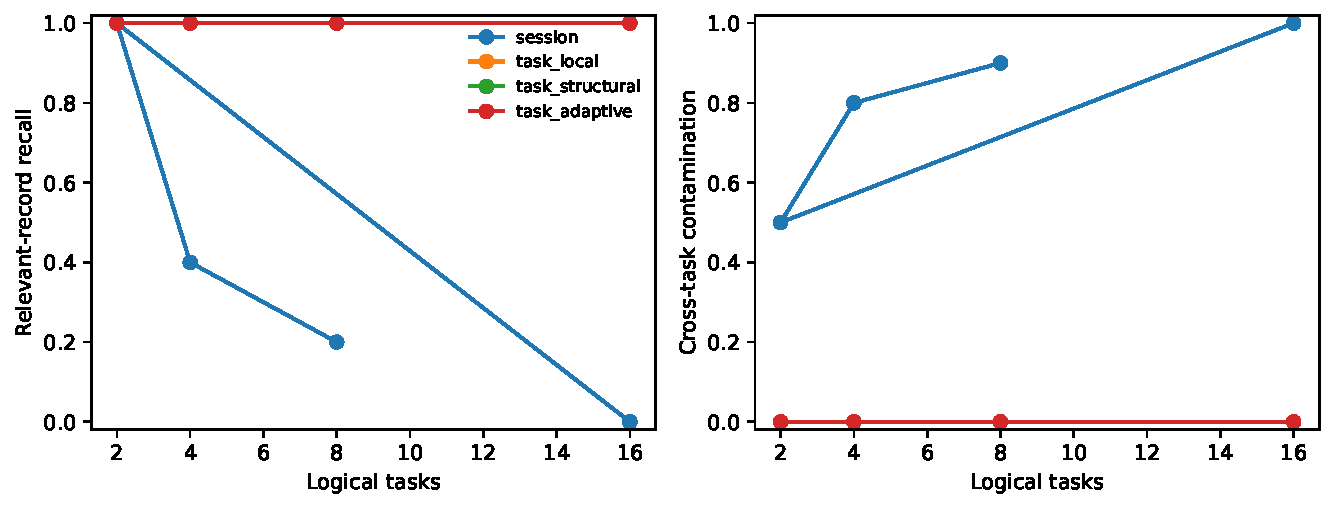
\includegraphics[width=\linewidth]{../shared/figures/paper8_tasks/task_scaling.pdf}
  \caption{Oracle parallel-workflow scaling under a matched record budget. Session-wide ranking increasingly selects recent, semantically similar records from the wrong task. Task-aware admission preserves active-task recall and removes cross-task contamination in this controlled construction.}
  \label{fig:task-scaling}
\end{figure}

\begin{figure}[t]
  \centering
  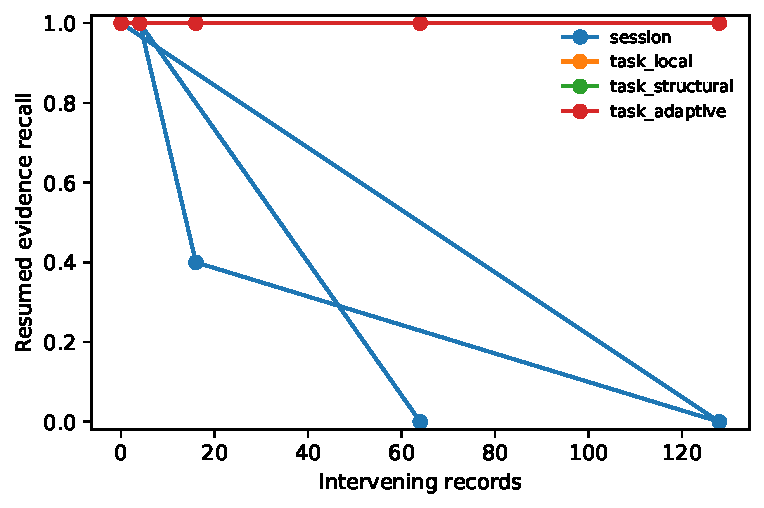
\includegraphics[width=0.72\linewidth]{../shared/figures/paper8_tasks/task_resumption.pdf}
  \caption{Resuming the oldest task after increasing intervening history. Task-local, structural, and adaptive scope preserve the required record; session-wide ranking is displaced by recent wrong-task evidence.}
  \label{fig:resumption}
\end{figure}

\section{Results}
Figure~\ref{fig:task-scaling} shows the central mechanism result. Averaged across the four parallel task counts, session-wide recall is 0.40 and contamination is 0.80. All three task-aware policies reach 1.00 recall and zero contamination. At 16 tasks the contrast is complete: session-wide recall is zero and contamination is one; every task-aware scope has recall one and contamination zero. Each selected set contains two records and 42 serialized visible tokens, so the difference is admission rather than a larger active context.

\begin{table}[t]
\centering
\caption{Sixteen-task parallel condition, mean over five seeds. $R$ is relevant-record recall, $P$ useful precision, and $C$ cross-task contamination.}
\label{tab:parallel16}
\begin{tabular}{lrrr}
\toprule
Policy & $R$ & $P$ & $C$ \\
\midrule
PRA\_SESSION & 0.00 & 0.00 & 1.00 \\
PRA\_TASK\_LOCAL & 1.00 & 0.50 & 0.00 \\
PRA\_TASK\_STRUCT & 1.00 & 0.50 & 0.00 \\
PRA\_TASK\_ADAPTIVE & 1.00 & 0.50 & 0.00 \\
\bottomrule
\end{tabular}
\end{table}

Hard isolation is insufficient when work depends on earlier tasks. Table~\ref{tab:joins} reports the eight-input join. Local scope sees only the active join task and recovers one of eight required records. Structural closure admits all explicit predecessors and recovers every input. Session scope also succeeds in this construction because the budget equals the relevant set, but it considers the complete session rather than using known graph structure. Across all join sizes, local join completeness is zero. Structural and session completeness is 0.75 because the 16-input case exceeds the eight-record cap.

\begin{table}[t]
\centering
\caption{Eight-input join, mean over five seeds. $J$ is complete recovery of every predecessor input.}
\label{tab:joins}
\begin{tabular}{lrrr}
\toprule
Policy & Recall & Precision & $J$ \\
\midrule
PRA\_SESSION & 1.000 & 1.000 & 1.00 \\
PRA\_TASK\_LOCAL & 0.125 & 0.167 & 0.00 \\
PRA\_TASK\_STRUCT & 1.000 & 1.000 & 1.00 \\
PRA\_TASK\_ADAPTIVE & 1.000 & 1.000 & 1.00 \\
\bottomrule
\end{tabular}
\end{table}

Figure~\ref{fig:resumption} gives the resumption result. At 128 intervening records, session-wide recall is zero with contamination one; every task-aware policy retains recall one and contamination zero. The lifecycle control independently verifies that switching away from a hot 128-token wrong-task working set demotes all 128 tokens before promoting 64 active-task tokens. This is state-transition accounting, not a measured GPU transfer.

\begin{figure}[t]
  \centering
  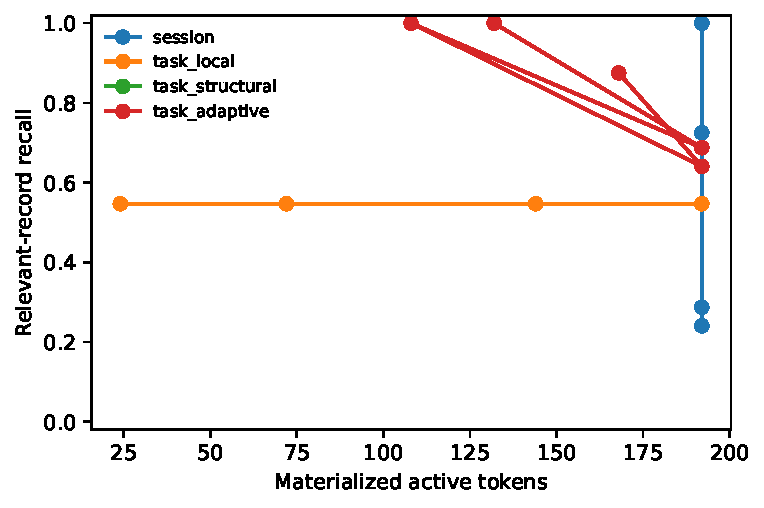
\includegraphics[width=0.72\linewidth]{../shared/figures/paper8_tasks/scope_detail_frontier.pdf}
  \caption{Scope breadth and materialization depth under a 192-token allowance. Structural scope spends the same or fewer charged tokens than session scope while recovering more relevant records at deeper views. Hard local scope is cheap but loses join inputs.}
  \label{fig:frontier}
\end{figure}

The scope--detail frontier in Figure~\ref{fig:frontier} makes the two-axis decomposition operational. At selected detail, structural scope averages 0.875 recall using 168 charged tokens, versus 0.725 recall and 192 tokens for session scope. At native-K/V depth, structural scope reaches 0.641 recall at 192 tokens versus 0.241 for session scope. Local scope uses fewer tokens when the candidate partition is small, but its aggregate recall is 0.547 because joins require predecessor evidence. These estimates validate accounting and policy behavior; they are not measurements of model-native K/V byte transfer.

\section{Interpretation and Limits}
The experiment establishes that explicit task structure can alter which records receive a fixed PRA budget, and that structural closure repairs the dependency loss caused by hard local filtering. It does not establish downstream answer accuracy, planning quality, or production latency. The semantic confusability is synthetic and deliberately severe. The lexical/recency ranker is a frozen control, not a competitive learned router.

Capacity remains a hard limit. In the 16-input join, an eight-record budget yields 0.50 recall and zero complete joins for structural, adaptive, and session policies. Task scope removes irrelevant competition; it cannot fit more required evidence than the materialization budget. Adaptive widening also equals structural scope in the primary cases because oracle metadata is complete. Its value under missing or stale metadata remains unmeasured.

The JSON and Markdown parser fixtures pass deterministic validation, but no language model produced those plans. Online tools and hybrid acquisition are explicitly marked deferred in the artifact bundle. The next empirical gate is model answer/action evaluation under oracle task structure, followed by metadata corruption and only then generated preflight plans.

\section{Hypotheses}
\begin{enumerate}[label=H\arabic*.]
\item Interleaving degrades session-wide PRA faster than task-aware PRA.
\item Explicit task scope reduces cross-task contamination without materially reducing required-evidence recall.
\item Gains increase with semantic similarity and hot-state contamination among tasks.
\item Structural closure outperforms hard task-local scope on dependency and join workflows while remaining cheaper than session-global retrieval.
\item Explicit dependency relations outperform rediscovery of known dependencies.
\item Task completion is an effective context-demotion boundary when compact result views retain full backing addressability.
\item Task-conditioned working sets remain bounded/sublinear as total session history grows.
\item Task-aware gains increase with workflow width, depth, joins, resumption distance, and interleaving complexity.
\item Preflight decomposition can recover much of the oracle task-aware gain for models that do not reliably manage tasks online.
\item JSON and Markdown decomposition have model-dependent reliability; downstream utility matters more than exact graph match.
\item Hybrid preflight-plus-online mutation is useful only if online changes add genuine execution-discovered structure rather than noise.
\end{enumerate}

\section{Experimental Discipline}\label{sec:discipline}
The causal order is mandatory:
\begin{enumerate}
\item Given oracle task identity/relations, does task-aware scope improve PRA?
\item How does the gain scale with workflow/interleaving complexity?
\item How robust is it to imperfect/stale task metadata?
\item Can preflight decomposition recover useful structure?
\item Can online model-managed tasks match or improve preflight structure?
\item Does the hybrid justify its complexity?
\end{enumerate}

Do not confound task extraction/planning competence with the core PRA mechanism.

\section{Falsification}
Weaken the thesis if session-wide PRA matches task-aware PRA at matched budget under strong interleaving; structural closure loses essential evidence or widens to near-global scope; scope/materialization bookkeeping costs approach the savings; completed-task demotion harms downstream execution; task-aware gains vanish on DAG/join workflows; metadata errors make the system too brittle; preflight decomposition costs more than it saves; generated task graphs do not improve downstream context selection; or gains occur only on synthetic task labels.

\section{Implementation Status and Next Gates}
\begin{center}
\small
\begin{tabularx}{\linewidth}{@{}clX@{}}
\toprule
Phase & Status & Artifact or remaining gate \\
\midrule
A & Complete & Paper-7 records, views, backing, and cache lifecycle reused. \\
B & Complete & Versioned task graph, replay, provenance, and structural closure. \\
C & Complete & Four matched-budget scope policies with a frozen ranker. \\
D & Partial & Cold/warm/hot accounting complete; physical GPU transfer unmeasured. \\
E & Complete & Complexity, joins, resumption, contamination, and frontier artifacts. \\
F & Partial & Gate and JSON/Markdown validation exist; model evaluation has not run. \\
G & Deferred & Online task tools remain behind the oracle stop gate. \\
H & Deferred & Hybrid acquisition follows separate preflight and online evaluation. \\
\bottomrule
\end{tabularx}
\end{center}

\section{Roadmap Boundary}
Paper~8 remains single-session and does not introduce subagent context trees, cross-session memory, or a new general planner. Paper~9 extends the context topology to separate-session subagents. Paper~10 studies cross-session memory.

\section{Target Claim}
The paper does not claim invention of task lists, workflow DAGs, task planning, or decomposition prompting. Its target claim is:

\emph{Explicit typed task state and workflow relations can serve as a first-class context-scope signal, allowing PRA to reconstruct bounded logical task contexts from an interleaved physical session while reusing ordinary PRA discovery and progressive materialization, and while keeping authoritative execution state in the harness.}

\end{document}
